\subsection{Cone}

\begin{figure}[H]
    \centering
    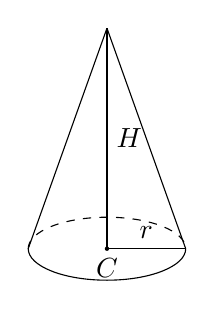
\begin{tikzpicture}[scale=0.8]
        \draw (0,0) -- (-1.25,-3.5);
        \draw (-1.25,-3.5) arc (180:360:1.25 and 0.5);
        \draw [dashed] (-1.25,-3.5) arc (180:360:1.25 and -0.5);
        \draw (1.25,-3.5) -- (0,0);  
        \draw (0,-3.5) -- node[anchor=west] { $H$ } (0,0);  
        \draw (0, -3.5) -- node[anchor=south] { $r$ } (1.25, -3.5);
        \fill (0, -3.5) circle [radius=1pt] node[anchor=north] { $C$ };
    \end{tikzpicture}
\end{figure}

\subsubsection{Area}

\[
    A = \pi r^2 + \pi r\sqrt{r^2 + H^2}
\]

\subsubsection{Volume}

\[
    V = \frac{1}{3}\pi r^2 H
\]



